\section{Vorwort}

Hallo liebe Stammesköche,~\\
~\\
seid ihr schon aufgeregt? Wir schon! Damit auch wirklich nix schiefgeht und ihr genau wisst, was ihr mit den ganzen Zutaten, die ihr von uns bekommt, anfangen könnt, haben wir für euch dieses Kochbuch vorbereitet.\\
~\\
In den Rezepten stehen immer die Mengen für 10 Personen. Ihr müsst aber eigentlich eh nichts umrechnen – ihr kriegt ja von uns genau das, was ihr braucht. ~\\
~\\
Zu den Brotmahlzeiten gibt es immer Wurst, Käse, Aufstriche, Gemüse, Obst, etc. – wenn ihr merkt, dass ihr bspw. zu viel Wurst habt, sagt es uns. Wir heben sie im Kühlschrank für euch auf und wenn ihr sie erst abends braucht, bekommt ihr sie dann. ~\\
~\\
Wir alle wissen, dass man eine Menge Zeit in der Küche totschlägt, bis das Wasser kocht, die Kisten kommen oder alles geschnibbelt ist. Damits euch nicht zu lang wird, birgt dieses Kochbuch noch einiges mehr als Rezepte.~\\
~\\
Falls ihr Fragen oder Lob habt, wendet euch vertrauensvoll an uns. Falls ihr meckern wollt, geht woanders hin – zur Technik oder so.~\\
~\\
Wir sehn uns,~\\
~\\
~~~~~Jonas, Kilian \& Anni~\\
~\\
P.S.: Risotto ist der Hit

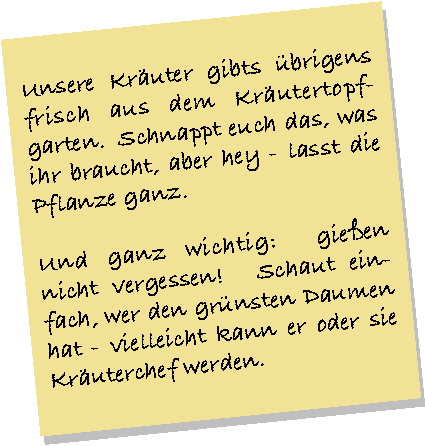
\includegraphics[right]{note-crop.pdf}